\documentclass{standalone}
\usepackage{tikz,ctex}
\usepackage{tikz-3dplot} % 2-1
\usepackage{unicode-math} % 2-5,4-1,4-2
\setmathfont{Fira Math Regular}
\setmainfont{Fira Sans}
\definecolor{background}{RGB}{239, 239, 239} % 4-5,6-2,6-5
\begin{document}
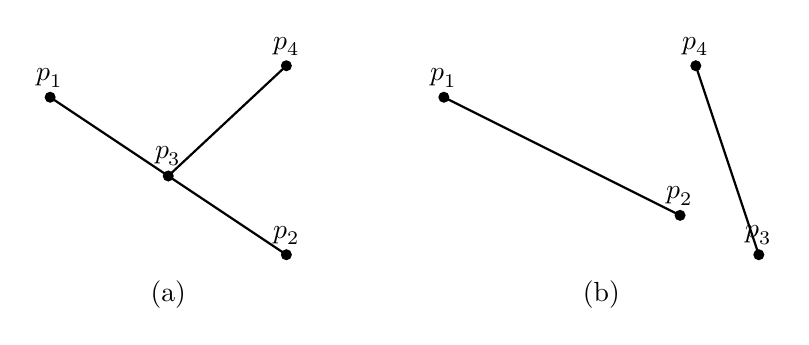
\begin{tikzpicture}
\foreach \x/\y[count=\i] in{0/2,3/0,1.5/1,3/2.4}{
    \fill (\x,\y) circle[radius=2pt] coordinate(\i) node[above]{$p_\i$};}
\foreach \u/\v in{1/2,3/4}{
    \draw[thick](\u)--(\v);}
 \node at(1.5,-.5) {(a)};
\foreach \x/\y[count=\i] in{5/2,8/.5,9/0,8.2/2.4}{
    \fill (\x,\y) circle[radius=2pt] coordinate(\i) node[above]{$p_\i$};}
\foreach \u/\v in{1/2,3/4}{
    \draw[thick](\u)--(\v);}
\node at(7,-.5) {(b)};
\end{tikzpicture}
\end{document}